\chapter{ Implementación}

\section{ Plataforma de desarrollo}
La plataforma para desarrollar la API ha sido un entorno basado en linux, concretamente\texttt{ Ubuntu 16.04LTS}. El Entorno de desarrollo elegido es \texttt{QT Creator} junto con \texttt{QT} 5.10.1. Y las librerías se apoyo son:
\begin{itemize}
	\item OpenGL 4.5.
	\item OpenMesh 7.0.
	\item CMake 3.5.1
\end{itemize} 

Además se ha utilizado un control de versiones, \texttt{git} en este caso, y para la parte de diagramas, esquemas e Ingeniería del Software la plataforma \texttt{Draw.io}. 
 
\section{ Instalación y configuración}

\subsection{ Entorno de desarrollo}
\textbf{OpenGL 4.5}
\begin{enumerate}
	\item Para conseguir la última versión de OpenGL es necesario instalar los drivers de NVidia o de ATI (según tu tarjeta gráfica), y la última versión que sea compatible con Ubuntu. Ya que los controladores de la tarjeta gráfica viene con la API de OpenGL.
\end{enumerate} 

\newpage
\textbf{QT Creator y QT 5.10.1}
\begin{enumerate}
	\item Descargar el instalador de la \href{https://www.qt.io/download}{web oficial}.
	\begin{enumerate}
		\item Ejecutar el instalador y seguir los pasos, asegurandote de marcar para instalar QTCreator (en su versión actual) y QT 5.10.1., como se ve en la figura \ref{fig:qt_install_1.png}
		\item Seleccionar la ubicación de instalación en \texttt{/usr/local/qt}.
	\end{enumerate}
\end{enumerate} 

\begin{figure} %con el [H] le obligamos a situar aquí la figura
	\centering
	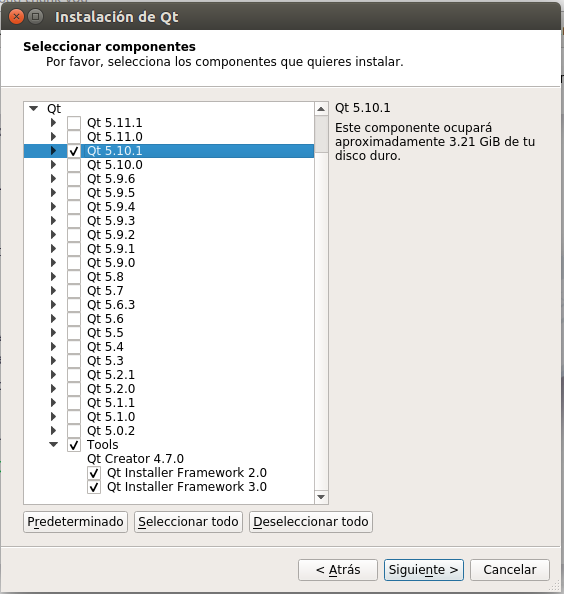
\includegraphics[scale=0.4]{imagenes/qt_install_1.png} 
	\caption{ Selección de paquetes a installar en QT installer.} \label{fig:qt_install_1.png}
\end{figure}

\textbf{OpenMesh}
\begin{enumerate}
	\item Descargar la API de OpenMesh desde \href{https://www.openmesh.org/download/}{sitio oficial}.
\end{enumerate} 	
	
	
\textbf{CMake}
\begin{enumerate}
	\item Installar CMake desde terminal y los repositorios de Ubuntu mediante el comando: \texttt{sudo apt-get install cmake}.
\end{enumerate} 



\subsection{ Configuración del Entorno}
Si has instalado QT después de tener actualizados o instalados los drivers de la tarjeta gráfica, el instalador debería de detectar que tienes instalado OpenGL e instala y configura los archivos necesarios para su funcionamiento. Además cuando se crea el proyecto con QT se debe de especificar en el archivo de configuración del proyecto (.pro) la siguiente línea:
\begin{lstlisting}[language=bash]
QT       += core gui opengl
\end{lstlisting}
para que lo compile usando la API de OpenGL.\\

Para configurar OpenMesh, es necesario tener instalado CMake, una vez comprobemos que está instalado seguimos los pasos de la documentación oficial de OpenMesh \href{URLhttps://www.openmesh.org/media/Documentations/OpenMesh-7.0-Documentation/a03933.html}{aquí}. Que nos indica según nuestro S.O. que pasos debemos seguir. Cuando se complete la configuración e instalación de OpenMesh es necesario que en el proyecto de QT en el archivo de configuración (.pro) se le indique que busqué las librerías de OpenMesh en el directorio donde lo hayamos instalado, en mi caso fue el siguiente:
\begin{lstlisting}[language=bash]
LIBS += \
/usr/local/lib/libOpenMeshCore.so  \
/usr/local/lib/libOpenMeshTools.so
\end{lstlisting}

Hay que indicar las dos librerías la \texttt{libOpenMeshCore.so} y la \texttt{libOpenMeshTools.so} ya que necesitaremos algunas de las tools que incluye, como son la lectura de ficheros PLY.

\section{ Desarrollo}

La estructura de datos es muy importante en este proyecto por ello se ha utilizado los contenedores de QT ya que viene con muchos métodos de ayuda y acceso a dichos contenedores además de traer incluidos unos iteradores para su navegación muy completos y eficientes. El contenedor principal del proyecto son las QLinkedList (\cite{QLinkedListClassQt}) ya que nos permiten una mejor gestión de la memoria y no es necesario que estén los elementos uno al lado de otro, así las eliminaciones e inserciones son muy rápidas y no afectan a las referencias que tiene unos elementos a otros puesto que cada uno siempre conserva su posición independientemente de las operaciones que se apliquen. Aunque el acceso a un elemento aleatorio es mejor con el vector y más eficiente los problemas que originan el borrado al desplazar los elementos para evitar la fragmentación interna de la memoria son mucho peores que en las listas, donde el acceso es de orden $O(n)$ pero el borrado mediante el puntero al objeto es de orden $O(1)$.

\subsection{ Input}
La clase input nos permite capturar los eventos producidos por el usuario a través del teclado y del ratón. De esta forma se le permite al usuario interactuar con la escena. La funcionalidad de esta clase es sencilla, y además cómo el tema principal del proyecto no es la interacción con el usuario, se optó por utilizar una ya creada.\\

La clase funciona como un controlador de flags, es decir, registra todas los eventos que produce el teclado y el ratón y asigna un estado a cada una de las teclas. De este modo cuando se pulsa una tecla se le asigna el flag de ``InputPressed'' y cuando se suelta pasa al flag de ``InputRelease''. Así se puede tener un control fácil de en que estado se encuentran las teclas. Para el ratón sigue la misma lógica, y además guarda la posición del puntero sobre la pantalla.

\subsection{ Camera3D}
La clase Camera3D contiene toda la lógica necesaria para crear una cámara y colocarla en la escena, como se explico en el capítulo 4, Análisis, la cámara es un factor muy importante de nuestro sistema, pero al igual que con la clase Input no es el principal tema del sistema por lo que también se optó por utilizar una ya existente, pero en ese casó si vamos a comentar los métodos más destacados así como su funcionalidad completa.\\

La clase contiene los atributos básicos de una cámara, que son: los vectores Dirección, Up y Right, además de la matriz con la rotación y traslación necesarias y por último una matriz con la transformación global del mundo. Todos estos atributos tienen sus métodos setter y getter sobrecargados para distintas opciones.\\

En cuanto a los métodos el más importante es de toMatrix(), ya que genera una matriz de proyección y restaura los flags que indican si hay alguna modificación pendiente.

\subsection{ Vertex}
Toda la lógica y modelo de los vértices se encuentra en esta clase, que posee los siguientes atributos:

\begin{itemize}
	\item \textit{m\_position: QVector3D}: representa a un vector 3D que indica la posición del vértice en el mundo de coordenadas de la escena.
	\item \textit{m\_color: QVector3D}: indica el color que posee el vértice en formáto RGB y con valor de 0 a 1. 
	
	\item \textit{halfEdgeIn: QLinkedList<HalfEdge>}: Es un conjunto de referencias a las semi-aristas que inciden sobre el vértice.
	\item \textit{halfEdgeOut: QLinkedList<HalfEdge>}: Es un conjunto de referencias a las semi-aristas que provienen del vértice.
\end{itemize}

Estos atributos son necesarios para facilitar la navegación por la malla. Poder saber qué semi-aristas salen o inciden sobre el vértice facilita mucho la gestión de las semi-aristas. Estos atributos junto con los de posición y color cuentan con los setter y getter habituales. En cuanto a los métodos principales de la clases se detallan a continuación.\\

\subsubsection*{positionOffset y colorOffset}
Indican el desplazamiento de las coordenadas de posición  y los valores de color en el objeto vértice. Cuando un objeto tiene varios atributos, estos se alojan en posiciones continuas en memoria y según el tipo de dato ocuparán más o menos posiciones. Por ejemplo el atributo posición de tipo float, ocupará 4 bytes y al ser una 3-tupla serán 12 bytes en total, tal como se refleja en el figura \ref{fig:vertex_attribute_pointer_interleaved.png}, donde se puede apreciar como las coordenadas X,Y y Z se alojan en la memoria en posiciones continuas. OpenGL provee un método para saber el offset del atributo de un objeto. Utilizando esta funcionalidad de OpenGL sabemos el offset exacto. El offset es importante  puesto que a la hora de alojar los datos en la GPU se debé indicar todos las coordenadas seguidas sin ningún dato entre medias, por ello OpenGL tiene la funcionalidad de indicarle el array de objectos y luego el offset del atributo en cuestión por si el objeto contiene más información, que suele ser lo habitual.\\

\subsubsection*{Stride}

Otro método importante requerido es el ``Stride'' que indica cuanto ocupa en memoria el objeto, para así poder saber cada cuanto espacio están separados los atributos, se puede apreciar más claramente en la figura \ref{fig:vertex_attribute_pointer_interleaved.png} con un ejemplo del array de vértices.


\begin{figure} %con el [H] le obligamos a situar aquí la figura
	\centering
	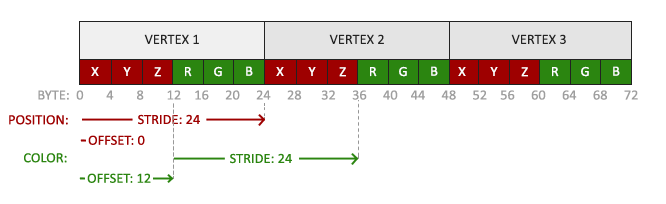
\includegraphics[scale=0.6]{imagenes/vertex_attribute_pointer_interleaved.png} 
	\caption{ Diagrama de un array de vértices, explicando gráficamente el offset y stride. Fuente de la imagen \url{https://learnopengl.com/Getting-started/Shaders}} \label{fig:vertex_attribute_pointer_interleaved.png}
\end{figure}



\subsection{ Face}
Toda la lógica y modelo de los vértices se encuentra en esta clase, que posee los siguientes atributos:

\begin{itemize}
	\item \textit{vértices: QVector<Vertex>}: representa el conjunto de vértices que forma la cara.
	\item \textit{normal: QVector3D}: vector unitario que representa la normal de la cara. Tiene el formato de 3-tupla de reales.
	\item \textit{MAX\_POSITION: Integer}: variable de control que indica el máximo número de elementos del vector vértices, así se controla que una cara o triángulo no esté formado por más de tres vértices.
\end{itemize}

Los principales métodos de esta clase se detallan a continuación.

\subsubsection*{remplaceVertex(Vertex \&\_vertexOld, Vertex \&\_vertexNew)}

RemplaceVertex pertmite dado un vértice remplazarlo por otro, para ello es necesario recorrer los vértices que forman la cara y buscar el vértice a sustituir por su atributo \texttt{id} y se sustituye.

\subsubsection*{generateSurfaceNormal}
Esta funcionalidad genera una nueva normal de cara y la asigna al atributo. Es recomendable lanzarla después de actualizar alguno de los valores del objeto, pero no se llama después de cada modificación de forma automática para que en la creación del objeto no se llame hasta que no esté totalmente creado y así dejar esta responsabilidad al programador. El método está basado en el pseudo-código de la wiki de Khronos \cite{CalculatingSurfaceNormal}.\\

El proceso para calcular la normal consiste en el siguiente proceso:\\

$$A = (x,y,z)$$ 
$$B = (x,y,z)$$ 
$$C = (x,y,z)$$
Donde $A,B,C$ son los vértices que forman la cara.
\vspace{0.3cm}
$$\overrightarrow{U} = A - B$$
$$\overrightarrow{V} = C - B$$
Obtenemos los vectores dirección $U,V$, que tiene que partir del mismo vértice (figura \ref{fig:productovectorial.png}). Ahora aplicamos el producto vectorial entre los vectores $U$ y $V$ para obtener el vector perpendicular al plano que forman. Aquí se añade una corrección respecto al algoritmo original, y es que se aumentan proporcionalmente ambos vectores, de esta forma se elimina el fallo de los decimales en el procesador, puesto que si son números muy pequeños donde los decimales son de ordenes muy bajos puede ser que con el redondeo y la discretización que aplica el ordenador se causen errores considerables.
Ahora si se puede aplicar el producto vectorial.
\begin{figure} %con el [H] le obligamos a situar aquí la figura
	\centering
	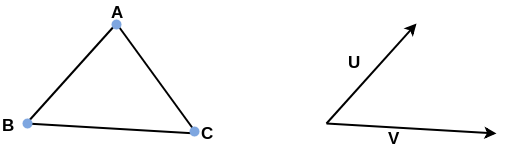
\includegraphics[scale=0.4]{imagenes/productovectorial.png} 
	\caption{Resultado de Restar los Vértices A - B y C - B} \label{fig:productovectorial.png}
\end{figure}

\[ 
N = \overrightarrow{U} \times \overrightarrow{V} = \begin{bmatrix}
i & j & k \\
U_x & U_y & U_z \\
V_x & V_y & V_z 
\end{bmatrix}  
\]

\vspace{0.3cm}

$$\overrightarrow{N_x} = \overrightarrow{U_y}*\overrightarrow{V_z} - (\overrightarrow{U_z}*\overrightarrow{V_y})$$
$$\overrightarrow{N_y} = \overrightarrow{U_z}*\overrightarrow{V_x} - (\overrightarrow{U_x}*\overrightarrow{V_z})$$
$$\overrightarrow{N_z} = \overrightarrow{U_x}*\overrightarrow{V_y} - (\overrightarrow{U_y}*\overrightarrow{V_x})$$

Ahora es necesario aplicar una normalización del vector normal. Esto se realiza mediante la división del módulo unidad del vector.

$$ ||N|| = \sqrt{N_x^2 + N_y^2 + N_z^2}$$

\begin{center}
$ N_x = \frac{N_x}{||N||}$
$ N_y = \frac{N_y}{||N||}$
$ N_z = \frac{N_z}{||N||}$
\end{center}


Una vez normalizado. Hay que ajustar los ejes por si alguna coordenada esta en negativo que es normal en el mundo 3D, pero en el vector de cara tiene que ser positivo. Así pues se calcula la normal de cara.

\newpage
\subsection{ HalfEdge}
Es una de las clases más importantes del proyecto, ya que alberga una de las funcionalidades más importante. Los atributos que la define, son muy parecidos a los descritos anteriormente:

\begin{itemize}
	\item \textit{vertexIn: Vertex}: referencia al vértice sobre el que incide la semi-arista.
	\item \textit{vertexOut: Vertex}: referencia al vértice del que proviene la semi-arista.
	\item \textit{face: Face}: una referencia a la cara adyacente, o que está formada en parte por la semi-arista.
	\item \textit{next: HalfEdge}: referencia a la semi-arista siguiente.
	\item \textit{previous: HalfEdge}: referencia a la semi-arista anterior.
	\item \textit{oposite: HalfEdge}: referencia a la semi-arista opuesta.
	\item \textit{errorRemove: Float}: indica el valor del error que produce si se elimina la semi-arista.
\end{itemize}

Los métodos de la clase son los típicos setter y getter, ya que esta clase cumple completamente con el patrón MVC y con su categoría de modelo.

\subsection{ Malla}
La clase malla es otra de las clases más importante del proyecto ya que contiene toda la lógica de la malla de triángulos. Los atributos que forman esta clase son:

\begin{itemize}
	\item \textit{vertices: QLinkedList<Vertex>}: un array de referencias a los vértices que componen la malla.
	\item \textit{sg\_vertices: QVector<Vertex>}: es un array de referencias ordenado de los vértices de la malla. Cada tres vértices indican las caras.
	\item \textit{indices: QLinkedList<Face>}: un conjunto de referencias a las caras que forman la malla.
	\item \textit{half\_edges:  QLinkedList<HalfEdge>}: conjunto de referencias a las semi-aristas que forman la malla.
\end{itemize}

Aunque los atributos sean pocos la organización del proyecto en distintas clases y métodos ha facilitado la composición de esta clase. Además el único atributo un poco más especial es el \textit{sg\_vertices} el cual contiene una referencia a los vértices ordenados para formar la malla. Esto es así para poder pasarle este vector de vértices a OpenGL y que el genere la malla. OpenGL tiene que recibir como parámetro un listado de vértices ordenados de tres en tres para generar las caras. En la figura \ref{fig:sgvertices.png} se puede observar cómo se colocan los vértices en dicho array para su correcta interpretación por parte de OpenGL. Es cierto que esta forma requiere más memoria que otras analizadas, pero con los equipos actuales, la utilización de referencias y la optimización de OpenGL a la hora de colocar los datos en las GPU se ha considerado que es una buena opción para nuestro caso. Además de los típicos setter y getter para todas las colecciones de objetos cabe destacar los siguientes métodos:\\

\begin{figure} %con el [H] le obligamos a situar aquí la figura
	\centering
	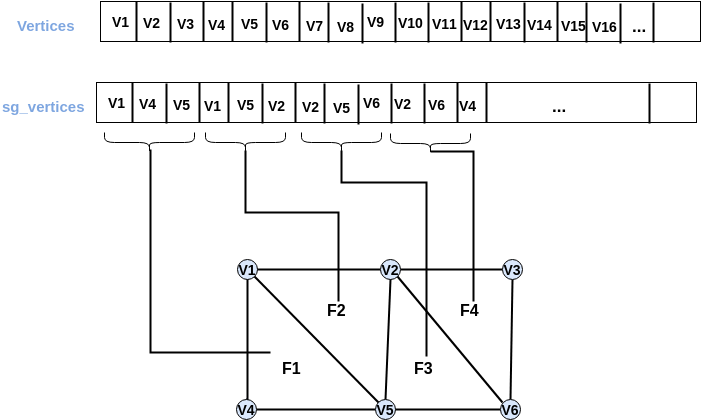
\includegraphics[scale=0.4]{imagenes/sgvertices.png} 
	\caption{Esquema de funcionamiento del atributo sg\_vertices conforme a lo establecido en OpenGL} \label{fig:sgvertices.png}
\end{figure}

\subsubsection*{initGeometry(string \_filename)}

La principal funcionalidad de este método es la de cargar una malla PLY en la estructura de datos interna. Para ello se hace uso de la API de OpenMesh, que nos permite leer un fichero PLY y cargarlo en su estructura de datos propia. Ahora la complejidad es pasar de la estructura de datos de OpenMesh a la propia, ya que la de OpenMesh utiliza muchos atributos más que no son requeridos para el proyecto y por tanto es espacio que conseguimos ahorrar. El proceso detallado es el siguiente:

\begin{enumerate}
	\item Cargar los vértices, OpenMesh contiene los vértices mediante una clase Handler y que se accede a través de iteradores. Una vez tenemos los iteradores consultamos la malla de OpenMesh solicitándole el vértice que apunta el iterador. Ya solo falta guardarlo en nuestro array particular de vértices.
	
	\item Cargar las caras, las caras son una secuencia de las posiciones de los vértices en grupos de tres que indican qué vértices forman la cara. Así pues la forma de conseguir esta secuencia se realiza mediante el id. Cada vértice añadido se le ha dado un id, que es un número desde el 0 hasta el número de vértices totales, de esta forma el vértice 0, tiene el id 0, y el vértice n, tiene el id n. Esto se cumple para el estado inicial, si se produce alguna alteración en el vector de vértices esta regla ya no se garantiza, pero para este caso sí. Entonces se recorre el listado de caras de OpenMesh y luego dentro de cada cara se coge el vértice de nuestro array con en la posición que marca los indices de la cara de OpenMesh.\\
	
	Además en este momento se calcula la normal de cara conforme de crea la cara en mi estructura.
	
	\item Semi-aristas aladas, las semi-aristas del mismo modo que los elementos anteriores se les asigna un id al crearlos y también están guardados en clases handler pero en este caso las semi-aristas contiene mucha información de los elementos anteriores, vértices y caras. Para ello se repite el proceso de recorrerlas con los iteradores y sacar la información deseada. A continuación se obtiene las caras mediante los métodos que nos provee OpenMesh que nos permiten consultar la posición de la cara mediante el iterador de la semi-aristas, así que aprovechando la propiedad descrita anteriormente de los id, se inicializa la cara incidente, los vértices sobre el que incide la semi-arista y el vértice del que parte.\\
	
	Por último una vez guardadas todas las semi-aristas se procede a asignar las semi-aristas de referencia, la siguiente, la anterior y la posterior. Volviendo a aprovechar la propiedad de los id pero esta vez con las semi-aristas, ya que OpenMesh nos vuelve a indicar las referencias mediante los ids.
	
	\item Como último paso es generar la geometría de la malla, esto se realiza con el método de generateGeometry.
	 
\end{enumerate}

\subsubsection*{generateGeometry}
Genera la geometría de la malla mediante la inicialización del vector sg\_vertices. Para ello recorro el listado de caras y dentro de cada cara se recorre el listado de sus tres vértices. Ahora solo hay que añadir los vértices en el vector de sg\_vertices. De esta forma simple se inicializa el vector.


\subsection{Connectivity}

La clase Connectivity no posee atributos como tal, ya que es la encargada de encapsular los algoritmos de procesado geométrico, por ello suelen recibir como parámetro la malla sobre la que aplicar el algoritmo y otros parámetros de configuración.

\subsubsection*{angleVector( u, v, resultado)}
La funcionalidad de este método es la de calcular el ángulo que forman los vectores $U$ y $V$ y guardar el resultado en la variable ``resultado''. Básicamente el método realiza un producto cruzado para obtener el angulo en radianes. Si el resultado fuera una indeterminación se aplica un valor alto.

\subsubsection*{calcOneRingError( halfedge)}
Método que calcula el error que produciría si se eliminase la arista pasada por parámetro. Realiza dicho cálculo y lo asigna al atributo de la semi-arista. El cálculo de error de un anillo de distancia se explicó en el capitulo 4, Análisis, y se ha implementado tal y como se espera.

\newpage
\subsubsection*{collapse (halfedge, Malla)}
Es uno de los métodos principales del proyecto y realiza una simplificación de una arista, junto con las dos caras a la que delimita y el vértice origen de la misma. La semi-arista dada como parámetro define la dirección y que vértice se colapsa con quién, mediante los atributos \textit{vertexIn} y \textit{vertexOut}. El proceso de collapse se define por el siguiente pseudo-código:

\begin{lstlisting}[frame=single]
h = semi-arista a eliminar;
hn = semi-arista siguiente a h;
hp = semi-arista anterior a h;

o = semi-arista opuesta a h;
on = semi-arista siguiente a o;
op = semi-arista anterior a o;

vh = vertice sobre el que incide h;
vo = vertice origen de h;

mesh.eliminaCara(h.getCara());
mesh.eliminaCara(o.getCara());

// Re-estructuracion de las referencias de las semi-aristas opuestas de las caras eliminadas.
hn.getOposite().getOposite() = hp.getOposite();
hp.getOposite().getOposite() = hn.getOposite();

on.getOposite().getOposite() = op.getOposite();
op.getOposite().getOposite() = on.getOposite();

// Eliminar las referencias a las semi-aristas en los vertices
hn.getVertexIn().removeHalfEdge(hn);
hn.getVertexOut().removeHalfEdge(hn);

hp.getVertexIn().removeHalfEdge(hp);
hp.getVertexOut().removeHalfEdge(hp);

h.getVertexIn().removeHalfEdge(h);
h.getVertexOut().removeHalfEdge(h);

on.getVertexIn().removeHalfEdge(on);
on.getVertexOut().removeHalfEdge(on);

op.getVertexIn().removeHalfEdge(op);
op.getVertexOut().removeHalfEdge(op);

o.getVertexIn().removeHalfEdge(o);
o.getVertexOut().removeHalfEdge(o);

mesh.remove(hn,hp,on,op);

// Las semi-aristas que inciden sobre vo ahora inciden sobre vh
for(HalfEdge he: vo.AllHalfEdgeIn){
	he.setVertexIn(vo);
	vh.addHalfEdgeIn(he);
}

// Las semi-aristas que tiene origen sobre vo ahora lo tienen sobre vh
for(HalfEdge he: vo.AllHalfEdgeOut){
	he.setVertexIn(vo);
	vh.addHalfEdgeIn(he);
}

mesh.getCaras.remplazar(vo,vh);
mesh.getCaras.recalcularNormaldeCaras();

mesh.getAllHalfEdges.remove(h,o);
mesh.getAllVertices.remove(vo);

\end{lstlisting}

De la línea 16 a la línea 20 se realiza una re-estructuración muy importante para la continuidad de la malla. Esta parte del proceso es delicada ya que requiere que las caras que se van a eliminar mantengan las propiedades en el resto por lo tanto se aplica que la semi-aristas opuestas que se van a eliminar se enlacen con las semi-aristas opuestas de las semi-aristas siguientes. Para entenderlo de forma más fácil ver la figura \ref{fig:collapse_011.png}, donde las semi-aristas opuestas a hn y hp son hn.O y hp.O respectivamente. Después de eliminar las caras 0 y 1, las opuestas de hn.O y hp.O estarán apuntando a posiciones vacías y por tanto ya no se mantendrían las propiedades de la malla. Así que se asignan las hn.O y hp.O como opuestas entre sí manteniendo la concordancia entre caras.

\begin{figure} %con el [H] le obligamos a situar aquí la figura
	\centering
	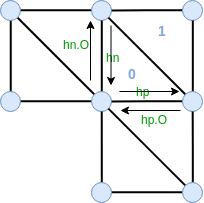
\includegraphics[scale=0.8]{imagenes/collapse_011.png} 
	\caption{Esquema de re-estructuración de semi-aristas opuestas en el método collapse. En Azul las caras y en Verde las semi-aristas.} \label{fig:collapse_011.png}
\end{figure}

\newpage
\subsubsection*{generateLowerErrorQueue( Malla, PriorityQueue)}

Este es otro de los métodos fundamentales del procesado geométrico ya que nos define una cola con prioridad de todas las semi-aristas de la malla de triángulos. La lógica de este método es la siguiente:

\begin{lstlisting}[frame=single]
priorityQueue.clear;

for(HalfEdge he: malla.getAllHalfEdges){
	calcOneRingError(he);
	priorityQueue.add(he);
}

\end{lstlisting}

Al crear una estructura de datos con bastante funcionalidad y encapsular los métodos la construcción de este método es más lógica que compleja.

\subsubsection*{decimation( Malla, tasaReducción)}
Y por último el método más importante del proyecto, donde se realiza la simplificación iterativa del collapse. Este método es el que enlaza toda la funcionalidad anterior y completa un flujo del proceso.
La lógica que sigue es la siguiente:

\begin{lstlisting}[frame=single]
num_reducciones = calcularNumeroReducciones(tasaReduccion);

generateLowerErrorQueue(pq);
HalfEdge he;

for(i=0 hasta num_reducciones){
	he = malla.getHalfEdge(pq.top());
	
	if(he.getFace != he.getOposite.getFace)
		collapse(he,malla);
	else
		mostrar error;
	
	pq.pop
	
	//Actualizamos los valores
	generateLowerErrorQueue(pq);
	
}
\end{lstlisting}

De esta forma el método de \textit{decimation} va reduciendo arista a arista hasta llegar a la tasa de reducción elegida y siempre reduciendo la arista que menos error produce, obteniendo así una malla optima en todo momento.